\documentclass{ximera}

%\usepackage{todonotes}

\newcommand{\todo}{}

\usepackage{esint} % for \oiint
\graphicspath{
{./}
{functionsOfSeveralVariables/}
{normalVectors/}
{lagrangeMultipliers/}
{vectorFields/}
{greensTheorem/}
{shapeOfThingsToCome/}
}


\usepackage{tkz-euclide}
\tikzset{>=stealth} %% cool arrow head
\tikzset{shorten <>/.style={ shorten >=#1, shorten <=#1 } } %% allows shorter vectors

\usetikzlibrary{backgrounds} %% for boxes around graphs
\usetikzlibrary{shapes,positioning}  %% Clouds and stars
\usetikzlibrary{matrix} %% for matrix
\usepgfplotslibrary{polar} %% for polar plots
\usetkzobj{all}
\usepackage[makeroom]{cancel} %% for strike outs
%\usepackage{mathtools} %% for pretty underbrace % Breaks Ximera
\usepackage{multicol}
\usepackage{pgffor} %% required for integral for loops


%% http://tex.stackexchange.com/questions/66490/drawing-a-tikz-arc-specifying-the-center
%% Draws beach ball
\tikzset{pics/carc/.style args={#1:#2:#3}{code={\draw[pic actions] (#1:#3) arc(#1:#2:#3);}}}



\usepackage{array}
\setlength{\extrarowheight}{+.1cm}   
\newdimen\digitwidth
\settowidth\digitwidth{9}
\def\divrule#1#2{
\noalign{\moveright#1\digitwidth
\vbox{\hrule width#2\digitwidth}}}





\newcommand{\RR}{\mathbb R}
\newcommand{\R}{\mathbb R}
\newcommand{\N}{\mathbb N}
\newcommand{\Z}{\mathbb Z}

%\newcommand{\sage}{\textsf{SageMath}}


%\renewcommand{\d}{\,d\!}
\renewcommand{\d}{\mathop{}\!d}
\newcommand{\dd}[2][]{\frac{\d #1}{\d #2}}
\newcommand{\pp}[2][]{\frac{\partial #1}{\partial #2}}
\renewcommand{\l}{\ell}
\newcommand{\ddx}{\frac{d}{\d x}}

\newcommand{\zeroOverZero}{\ensuremath{\boldsymbol{\tfrac{0}{0}}}}
\newcommand{\inftyOverInfty}{\ensuremath{\boldsymbol{\tfrac{\infty}{\infty}}}}
\newcommand{\zeroOverInfty}{\ensuremath{\boldsymbol{\tfrac{0}{\infty}}}}
\newcommand{\zeroTimesInfty}{\ensuremath{\small\boldsymbol{0\cdot \infty}}}
\newcommand{\inftyMinusInfty}{\ensuremath{\small\boldsymbol{\infty - \infty}}}
\newcommand{\oneToInfty}{\ensuremath{\boldsymbol{1^\infty}}}
\newcommand{\zeroToZero}{\ensuremath{\boldsymbol{0^0}}}
\newcommand{\inftyToZero}{\ensuremath{\boldsymbol{\infty^0}}}



\newcommand{\numOverZero}{\ensuremath{\boldsymbol{\tfrac{\#}{0}}}}
\newcommand{\dfn}{\textbf}
%\newcommand{\unit}{\,\mathrm}
\newcommand{\unit}{\mathop{}\!\mathrm}
\newcommand{\eval}[1]{\bigg[ #1 \bigg]}
\newcommand{\seq}[1]{\left( #1 \right)}
\renewcommand{\epsilon}{\varepsilon}
\renewcommand{\phi}{\varphi}


\renewcommand{\iff}{\Leftrightarrow}

\DeclareMathOperator{\arccot}{arccot}
\DeclareMathOperator{\arcsec}{arcsec}
\DeclareMathOperator{\arccsc}{arccsc}
\DeclareMathOperator{\si}{Si}
\DeclareMathOperator{\proj}{\vec{proj}}
\DeclareMathOperator{\scal}{scal}
\DeclareMathOperator{\sign}{sign}


%% \newcommand{\tightoverset}[2]{% for arrow vec
%%   \mathop{#2}\limits^{\vbox to -.5ex{\kern-0.75ex\hbox{$#1$}\vss}}}
\newcommand{\arrowvec}{\overrightarrow}
%\renewcommand{\vec}[1]{\arrowvec{\mathbf{#1}}}
\renewcommand{\vec}{\mathbf}
\newcommand{\veci}{{\boldsymbol{\hat{\imath}}}}
\newcommand{\vecj}{{\boldsymbol{\hat{\jmath}}}}
\newcommand{\veck}{{\boldsymbol{\hat{k}}}}
\newcommand{\vecl}{\boldsymbol{\l}}
\newcommand{\uvec}[1]{\mathbf{\hat{#1}}}
\newcommand{\utan}{\mathbf{\hat{t}}}
\newcommand{\unormal}{\mathbf{\hat{n}}}
\newcommand{\ubinormal}{\mathbf{\hat{b}}}

\newcommand{\dotp}{\bullet}
\newcommand{\cross}{\boldsymbol\times}
\newcommand{\grad}{\boldsymbol\nabla}
\newcommand{\divergence}{\grad\dotp}
\newcommand{\curl}{\grad\cross}
%\DeclareMathOperator{\divergence}{divergence}
%\DeclareMathOperator{\curl}[1]{\grad\cross #1}
\newcommand{\lto}{\mathop{\longrightarrow\,}\limits}

\renewcommand{\bar}{\overline}

\colorlet{textColor}{black} 
\colorlet{background}{white}
\colorlet{penColor}{blue!50!black} % Color of a curve in a plot
\colorlet{penColor2}{red!50!black}% Color of a curve in a plot
\colorlet{penColor3}{red!50!blue} % Color of a curve in a plot
\colorlet{penColor4}{green!50!black} % Color of a curve in a plot
\colorlet{penColor5}{orange!80!black} % Color of a curve in a plot
\colorlet{penColor6}{yellow!70!black} % Color of a curve in a plot
\colorlet{fill1}{penColor!20} % Color of fill in a plot
\colorlet{fill2}{penColor2!20} % Color of fill in a plot
\colorlet{fillp}{fill1} % Color of positive area
\colorlet{filln}{penColor2!20} % Color of negative area
\colorlet{fill3}{penColor3!20} % Fill
\colorlet{fill4}{penColor4!20} % Fill
\colorlet{fill5}{penColor5!20} % Fill
\colorlet{gridColor}{gray!50} % Color of grid in a plot

\newcommand{\surfaceColor}{violet}
\newcommand{\surfaceColorTwo}{redyellow}
\newcommand{\sliceColor}{greenyellow}




\pgfmathdeclarefunction{gauss}{2}{% gives gaussian
  \pgfmathparse{1/(#2*sqrt(2*pi))*exp(-((x-#1)^2)/(2*#2^2))}%
}


%%%%%%%%%%%%%
%% Vectors
%%%%%%%%%%%%%

%% Simple horiz vectors
\renewcommand{\vector}[1]{\left\langle #1\right\rangle}


%% %% Complex Horiz Vectors with angle brackets
%% \makeatletter
%% \renewcommand{\vector}[2][ , ]{\left\langle%
%%   \def\nextitem{\def\nextitem{#1}}%
%%   \@for \el:=#2\do{\nextitem\el}\right\rangle%
%% }
%% \makeatother

%% %% Vertical Vectors
%% \def\vector#1{\begin{bmatrix}\vecListA#1,,\end{bmatrix}}
%% \def\vecListA#1,{\if,#1,\else #1\cr \expandafter \vecListA \fi}

%%%%%%%%%%%%%
%% End of vectors
%%%%%%%%%%%%%

%\newcommand{\fullwidth}{}
%\newcommand{\normalwidth}{}



%% makes a snazzy t-chart for evaluating functions
%\newenvironment{tchart}{\rowcolors{2}{}{background!90!textColor}\array}{\endarray}

%%This is to help with formatting on future title pages.
\newenvironment{sectionOutcomes}{}{} 



%% Flowchart stuff
%\tikzstyle{startstop} = [rectangle, rounded corners, minimum width=3cm, minimum height=1cm,text centered, draw=black]
%\tikzstyle{question} = [rectangle, minimum width=3cm, minimum height=1cm, text centered, draw=black]
%\tikzstyle{decision} = [trapezium, trapezium left angle=70, trapezium right angle=110, minimum width=3cm, minimum height=1cm, text centered, draw=black]
%\tikzstyle{question} = [rectangle, rounded corners, minimum width=3cm, minimum height=1cm,text centered, draw=black]
%\tikzstyle{process} = [rectangle, minimum width=3cm, minimum height=1cm, text centered, draw=black]
%\tikzstyle{decision} = [trapezium, trapezium left angle=70, trapezium right angle=110, minimum width=3cm, minimum height=1cm, text centered, draw=black]

\outcome{Define the concept of a function.} 
\outcome{Distinguish between functions by considering their domains.}
\outcome{Plot basic functions.}
\outcome{Recognize different representations of the same function.}

\title[Dig-In:]{For each input, exactly one output}
\begin{document}
\begin{abstract}
  We define the concept of a function.
\end{abstract}
\maketitle


Life is complex. Part of this complexity stems from the fact that
there are many relationships between seemingly unrelated events. Armed
with mathematics, we seek to understand the world.  Perhaps the most
relevant ``real-world'' relation is
\begin{quote}
  \textbf{the position of an object with respect to time.}
\end{quote}
Our observations seem to indicate that every instant in time is
associated to a unique positioning of the objects in the universe.  You
may have heard the saying,
\begin{quote}
  \textbf{you cannot be two places at the same time,}
\end{quote}
and it is this fact that motivates our definition for functions.

\begin{definition}\index{function}
A \dfn{function} is a relation between sets where for each input,
there is exactly one output.
\end{definition}

\begin{question}
  If our function is the ``position with respect to time'' of some
  object, then the input is
  \begin{multipleChoice}
    \choice{position}
    \choice[correct]{time}
    \choice{none of the above}
  \end{multipleChoice}
  and the output is
  \begin{multipleChoice}
    \choice[correct]{position}
    \choice{time}
    \choice{none of the above}
  \end{multipleChoice}
\end{question}


Something as simple as a dictionary could be thought of as a relation,
as it connects \textit{words} to \textit{definitions}. However, a
dictionary is not a function, as there are words with multiple
definitions. On the other hand, if each word only had a single
definition, then a dictionary would be a function.

\begin{question}
  Which of the following are functions?
  \begin{selectAll}
    \choice{Mapping words to their definition in a dictionary.}
    \choice[correct]{Mapping social security numbers of living
      people to actual living people.}
    \choice[correct]{Mapping people to their birth date.}
    \choice{Mapping mothers to their children.}
  \end{selectAll}
  \begin{feedback}\hfil
    \begin{itemize}
    \item Since words may have more than one definition, ``relating
      words to their definition in a dictionary'' is not a function.
    \item Since every social security number corresponds exactly to
      one person, ``relating social security numbers of living people
      to actual living people'' is a function.
    \item Since every person only has one birth date, ``relating
      people to their birth date'' is a function.
      \item Since mothers can have more (or less) than one child,
        ``relating mothers to their children'' is not a function.
    \end{itemize}
  \end{feedback}
  
  \begin{warning}

Mapping people to their birth date is still a function, even though many people have the same birth date.  This is an instance of a function in which an output (a birth date) corresponds to many different inputs (people), but this mapping still a function because each input (person) has exactly one output (birth date).  Be careful: the only requirement for a function is that each input has exactly one output, not the other way around!

\end{warning}

\end{question}

What we are hoping to convince you is that the following are true:
\begin{enumerate}
\item The definition of a function is well-grounded in a real context.
\item The definition of a function is flexible enough that it can be
  used to model a wide range of phenomena.
\end{enumerate}




%% A function can be thought of as a ``mathematical machine.''
%% %% %%BADBAD Insert picture 1
%% This means for each input, there is exactly one output. 
%% %% %%BADBAD Insert picture 2


Whenever we talk about functions, we should explicitly state
what type of things the inputs are and what type of things the outputs
are.  In calculus, functions often define a relation from (a subset
of) the real numbers (denoted by $\RR$) to (a subset of) the real
numbers.

\begin{definition}
  We call the set of the inputs of a function the
  \dfn{domain}\index{domain}, and we call the set of the outputs of a
  function the \dfn{range}\index{range}.
\end{definition}

\begin{example}
Consider the function $f$ that maps from the real numbers to the real
numbers by taking a number and mapping it to its cube:
\begin{align*}
1 &\mapsto 1\\
-2 &\mapsto -8\\
1.5 &\mapsto 3.375
\end{align*}
and so on. This function can be \textit{described} by the formula
$f(x)=x^3$ or by the graph shown in the plot below:
\begin{image}
\begin{tikzpicture}
	\begin{axis}[
            domain=-2:2,
            width=6in,
            height=3in,
            axis lines =middle, xlabel=$x$, ylabel=$y$,
            every axis y label/.style={at=(current axis.above origin),anchor=south},
            every axis x label/.style={at=(current axis.right of origin),anchor=west},
          ]
	  \addplot [very thick, penColor, smooth] {x^3};
        \end{axis}
\end{tikzpicture}
%% \caption{A plot of $f(x)=x^3$. Here we can see that for each input (a
%%   value on the $x$-axis), there is exactly one output (a value on the
%%   $y$-axis).}
%% \label{plot:fxn x^3}
\end{image}
\end{example}

\begin{warning}
A function is a relation (such that for each input, there is exactly
one output) between sets. The formula and the graph are merely
descriptions of this relation.
\begin{itemize}
\item A formula \textbf{describes} the relation using symbols.
\item A graph \textbf{describes} the relation using pictures. 
\end{itemize}
The \textbf{function is the relation itself}, and is independent of how
it is described.  \\ For example, if $f(x) = x^2$ and $g(u) = u^2$, like on the previous card, $f = g$.  Even though these are two different formulas, they describe the same relation, so they are equal functions.
\end{warning}

Our next example may be a function that is new to you. It is the
\textit{greatest integer function}.

\begin{example}
Consider the \dfn{greatest integer function}.  This function maps
any real number $x$ to the greatest integer less than or equal to $x$.
%\[
%f(x) = \parbox{3in}{The function that maps any real number $x$
%  to the greatest integer less than or equal to $x$.}
%\]
People sometimes write this as $f(x) = \lfloor x\rfloor$, where those
funny symbols mean exactly the words above describing the
function. For your viewing pleasure, here is a graph of the greatest
integer function:
\begin{image}
\begin{tikzpicture}
	\begin{axis}[
            domain=-2:4,
            width=6in,
            height=3in,
            axis lines =middle, xlabel=$x$, ylabel=$y$,
            every axis y label/.style={at=(current axis.above origin),anchor=south},
            every axis x label/.style={at=(current axis.right of origin),anchor=west},
            clip=false,
            %axis on top,
          ]
          \addplot [textColor, very thin, domain=(0:2.3)] {0}; % puts the axis back, axis on top clobbers our open holes
          \addplot [textColor, very thin] plot coordinates {(0,0) (0,2)}; % puts the axis back, axis on top clobbers our open holes
	  \addplot [very thick, penColor, domain=(-2:-1)] {-2};
          \addplot [very thick, penColor, domain=(-1:0)] {-1};
          \addplot [very thick, penColor, domain=(0:1)] {0};
          \addplot [very thick, penColor, domain=(1:2)] {1};
          \addplot [very thick, penColor, domain=(2:3)] {2};
          \addplot [very thick, penColor, domain=(3:4)] {3};
          \addplot[color=penColor,fill=penColor,only marks,mark=*] coordinates{(-2,-2)};  %% closed hole          
          \addplot[color=penColor,fill=penColor,only marks,mark=*] coordinates{(-1,-1)};  %% closed hole          
          \addplot[color=penColor,fill=penColor,only marks,mark=*] coordinates{(0,0)};  %% closed hole          
          \addplot[color=penColor,fill=penColor,only marks,mark=*] coordinates{(1,1)};  %% closed hole          
          \addplot[color=penColor,fill=penColor,only marks,mark=*] coordinates{(2,2)};  %% closed hole  
          \addplot[color=penColor,fill=penColor,only marks,mark=*] coordinates{(3,3)};  %% closed hole                  
          \addplot[color=penColor,fill=background,only marks,mark=*] coordinates{(-1,-2)};  %% open hole
          \addplot[color=penColor,fill=background,only marks,mark=*] coordinates{(0,-1)};  %% open hole
          \addplot[color=penColor,fill=background,only marks,mark=*] coordinates{(1,0)};  %% open hole
          \addplot[color=penColor,fill=background,only marks,mark=*] coordinates{(2,1)};  %% open hole
          \addplot[color=penColor,fill=background,only marks,mark=*] coordinates{(3,2)};  %% open hole
          \addplot[color=penColor,fill=background,only marks,mark=*] coordinates{(4,3)};  %% open hole
        \end{axis}
\end{tikzpicture}
%% \caption{A plot of $f(x)=\lfloor x\rfloor$. Here we can see that for each input (a
%%   value on the $x$-axis), there is exactly one output (a value on the
%%   $y$-axis).}
%% \label{plot:greatest-integer fxn}
\end{image}
Observe that here we have multiple inputs that give
the same output.  This is not a problem! To be a function, we
merely need to check that for each input, there is exactly one output,
and this condition is satisfied.
\end{example}

\begin{question}
  Compute:
  \[
  \lfloor 2.4 \rfloor
  \begin{prompt}
    =\answer{2}
  \end{prompt}
  \]
  \begin{question}
  Compute:
  \[
  \lfloor -2.4 \rfloor
  \begin{prompt}
    =\answer{-3}
  \end{prompt}
  \]
\end{question}
\end{question}


Notice that both the functions described above pass the so-called
\textit{vertical line test}.  This test gives a quick visual check of whether each input (or $x$-value) corresponds to exactly one output (or $y$ value).

\begin{theorem}
The curve $y=f(x)$ represents $y$ as a function of $x$ at $x=a$ if and
only if the vertical line $x=a$ intersects the curve $y=f(x)$ at
exactly one point. This is called the \dfn{vertical line test}.
\end{theorem}

To use this test, imagine moving a vertical line over a graph starting on the left and then moving to the right.  If there is a vertical line $x=a$ that intersects the graph \textit{more than once}, then the input, $a$, corresponds to more than one output (or $y$-value), so the graph is \textit{not} the graph of a function.  On the other hand, if a vertical line can be moved over an entire graph and \textit{always} intersects the graph exactly once, then each input corresponds with exactly one output, so the graph is the graph of a function.

\begin{problem}
  Is the graph of the circle $y^2 = 4 - x^2$ shown below the graph of a function?
  
  \begin{center} 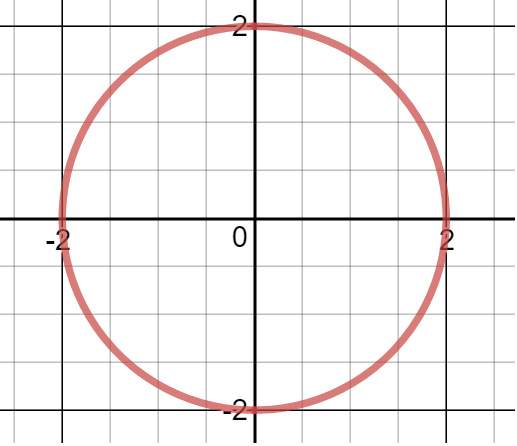
\includegraphics[scale=0.5]{functiondef1.png} \end{center}

  \begin{multipleChoice}
    \choice{yes}
    \choice[correct]{no}
  \end{multipleChoice}

  \begin{problem}
        Let's cut the previous circle in half.  Is the graph of the semi-circle $y = \sqrt{4 - x^2}$ shown below the graph of a function?
        
    \begin{center} 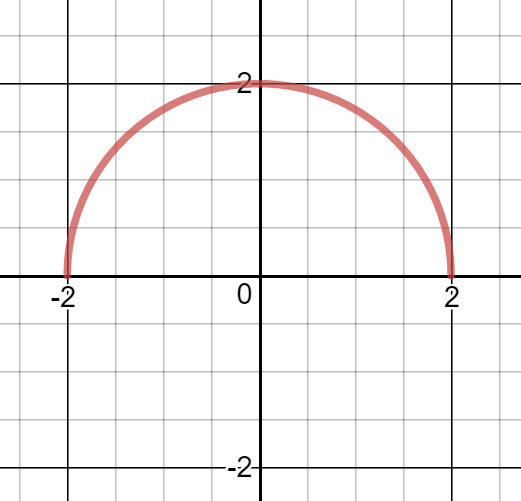
\includegraphics[scale=0.5]{functiondef2.png} \end{center}

    \begin{multipleChoice}
      \choice[correct]{Yes}
      \choice{No}
    \end{multipleChoice}
    \begin{feedback}[correct]
        Although the circle graph does not represent a function, the graph of the associated semi-circle does.  This semi-circle function is called a \textbf{branch} of the circle graph.
    \end{feedback}
  \end{problem}
\end{problem} 

Sometimes the domain and range are the \textit{entire} set of real
numbers, denoted by $\RR$. In our next examples we show that this is
not always the case.

\begin{example}
Consider the function that maps non-negative real numbers to their
positive square root. This function can be described by the
formula
\[
f(x) = \sqrt{x}.
\]
The domain is $0\le x<\infty$, which we prefer to write as
$[0,\infty)$ in interval notation. The range is $[0,\infty)$.  Here is
    a graph of $y=f(x)$:
\begin{image}
\begin{tikzpicture}
	\begin{axis}[
            xmin=-8,xmax=8,
            ymin=-5,ymax=5,
            width=6in,
            height=3in,
            domain=0:8,
            axis lines =middle, xlabel=$x$, ylabel=$y$,
            every axis y label/.style={at=(current axis.above origin),anchor=south},
            every axis x label/.style={at=(current axis.right of origin),anchor=west},
          ]
	  \addplot [very thick, penColor, smooth,samples=100] {sqrt(x)};
        \end{axis}
\end{tikzpicture}
%% \caption{A plot of $f(x)=\sqrt{x}$. Here we can see that for each
%%   input (a non-negative value on the $x$-axis), there is exactly one
%%   output (a positive value on the $y$-axis).}
%% \label{plot:sqrt fxn}
\end{image}
\end{example}

\begin{comment}

To really tease out the difference between a function and its
description, let's consider an example of a function with two
different descriptions.

\begin{example}
  Explain why $\sqrt{x^2} = |x|$.
  \begin{explanation}
    Although $\sqrt{x^2}$ may appear to simplify to just $x$, let's see
    what happens when we plug in some values.
    \[
    \begin{aligned}
    \sqrt{3^2} &= \sqrt{9}\\
    &=3,
    \end{aligned}
    \qquad\text{and}\qquad
    \begin{aligned}
      \sqrt{(-3)^2} &= \sqrt{9}\\
      &=3.
    \end{aligned}
    \]
    In an entirely similar way, we see that for any positive $x$, $f(-x)=\answer[given]{x}$.  Hence
    $\sqrt{x^2}\ne x$. Rather we see that $\sqrt{x^2} = |x|$.  The
    domain of $f(x)=\sqrt{x^2}$ is $(-\infty,\infty)$ and the range is
    $[0,\infty)$.  For your viewing pleasure we've included a graph of
      $y=f(x)$:
    \begin{image}
      \begin{tikzpicture}
	\begin{axis}[
            domain=-3:3,
            width=6in,
            height=3in,
            axis lines =middle, xlabel=$x$, ylabel=$y$,
            every axis y label/.style={at=(current axis.above origin),anchor=south},
            every axis x label/.style={at=(current axis.right of origin),anchor=west},
            xtick={-3,...,3},
            ytick={-3,...,3},
          ]
	  \addplot [very thick, penColor, domain=0:3] {x};
          \addplot [very thick, penColor, domain=-3:0] {-x};
        \end{axis}
      \end{tikzpicture}
    \end{image}
  \end{explanation}
\end{example}

\end{comment}

Finally, we will consider a function whose domain is all real numbers
except for a single point.

\begin{example}
  Are 
  \[
  f(x) = \frac{2x}{x} = 2 \cdot \frac{x}{x}
  \]
  and
  \[
  g(x) = 2
  \]
  the same function?
  \begin{explanation}
  Let's use a series of steps to think about this question. 
    First, what if we compare graphs? Here we see a graph of
    $f$:
    \begin{image}
      \begin{tikzpicture}
	\begin{axis}[
            domain=-3:3,
            axis lines =middle, xlabel=$x$, ylabel=$y$,
            every axis y label/.style={at=(current axis.above origin),anchor=south},
            every axis x label/.style={at=(current axis.right of origin),anchor=west},
            xtick={-2,...,2},
            ytick={-1,...,2},
          ]
	  \addplot [very thick, penColor, smooth] {2};
          \addplot[color=penColor,fill=background,only marks,mark=*] coordinates{(0,2)};  %% open hole
        \end{axis}
\end{tikzpicture}
%% \caption{A plot of $f(x)=\protect\frac{2x}{x}$. Here we
%%   can see that for each input (any value on the $x$-axis except for
%%   $x=0$), there is exactly one output (a value on the $y$-axis).}
%% \label{plot:point undfed fxn}
\end{image}
On the other hand, here is a graph of $g$:
\begin{image}
\begin{tikzpicture}
	\begin{axis}[
            domain=-2:2,
            axis lines =middle, xlabel=$x$, ylabel=$y$,
            every axis y label/.style={at=(current axis.above origin),anchor=south},
            every axis x label/.style={at=(current axis.right of origin),anchor=west},
            xtick={-2,...,2},
            ytick={-1,...,2},
          ]
	  \addplot [very thick, penColor, smooth] {2};
        \end{axis}
\end{tikzpicture}
%% \caption{A plot of $f(x)=\protect2$. 
\end{image}
Second, what if we compare the domains?  We cannot evaluate $f$ at
$x=\answer[given]{0}$.  This is the only $x$ value where $f$ is undefined, so the domain of $f$ is $\left(\infty, \answer[given]{0}\right) \ \bigcup \ \left(\answer[given]{0}, \infty\right)$.  On the other
hand, there is no value of $x$ where we cannot evaluate $g$.  In other
words, the domain of $g$ is $(-\infty, \infty)$ or $\RR$.

Since these two functions do not have the same graph and they do not
have the same domain, they must not be the same function.

However, if we look at the two functions everywhere except at $x = 0$, 
we can say that $f(x)=g(x)$.  In other words, 
\[
f(x)=2\qquad\text{when}\qquad \text{$x \ne 0$}.
\]
From this example we see that it is critical to consider the domain and
range of a function.
  \end{explanation}
\end{example}


\end{document}
